%%%%%%%%%%%%%%%%%%%%% chapter.tex %%%%%%%%%%%%%%%%%%%%%%%%%%%%%%%%%
%
% sample chapter
%
% Use this file as a template for your own input.
%
%%%%%%%%%%%%%%%%%%%%%%%% Springer-Verlag %%%%%%%%%%%%%%%%%%%%%%%%%%
%\motto{Use the template \emph{chapter.tex} to style the various elements of your chapter content.}
\chapter{Chapter Heading}
\label{intro} % Always give a unique label
% use \chaptermark{}
% to alter or adjust the chapter heading in the running head

\abstract*{Each chapter should be preceded by an abstract (no more than 200 words) that summarizes the content. The abstract will appear\textit{online} at \url{www.SpringerLink.com} and be available with unrestricted access. This allows unregistered users to read the abstract as a teaser for the complete chapter.
Please use the 'starred' version of the new \texttt{abstract} command for typesetting the text of the online abstracts (cf. source file of this chapter template\texttt{abstract}) and include them with the source files of your manuscript. Use the plain \texttt{abstract} command if the abstract is also to appear in the printed version of the book.}

\abstract{Each chapter should be preceded by an abstract (no more than 200 words) that summarizes the content. The abstract will appear \textit{online} at \url{www.SpringerLink.com} and be available with unrestricted access. This allows unregistered users to read the abstract as a teaser for the complete chapter. \newline\indent
Please use the 'starred' version of the new \texttt{abstract} command for typesetting the text of the online abstracts (cf. source file of this chapter template \texttt{abstract}) and include them with the source files of your manuscript. Use the plain \texttt{abstract} command if the abstract is also to appear in the printed version of the book.}

\section{Section Heading}
%\label{sec:1}
Use the template \emph{chapter.tex} together with the document class SVMono (monograph-type books) or SVMult (edited books) to style the various elements of your chapter content conformable to the Springer Nature layout.

\section{Section Heading}
%\label{sec:2}
% Always give a unique label
% and use \ref{<label>} for cross-references
% and \cite{<label>} for bibliographic references
% use \sectionmark{}
% to alter or adjust the section heading in the running head
Instead of simply listing headings of different levels we recommend to let every heading be followed by at least a short passage of text. Furtheron please use the \LaTeX\ automatism for all your cross-references and citations.



\abstract{Summarize Chapter Title}

\section{Attacker Privilege Escalation to Domain Administrator in Active Directory}

Advanced Techniques to Bypass Multi-Factor Authentication (MFA) Systems

Bypassing MFA is a critical subject for both offensive operators simulating real-world threats and defenders aiming to harden their authentication workflows. This technical guide explores modern MFA bypass methods with code examples and defensive recommendations.

1. Session Token Replay and Theft

Attack Overview:
Once a user completes MFA, the server issues a session token (e.g., cookie or JWT). If stolen, this token can be reused to impersonate the user without reauthentication.
(Python):
import requests 


Defensive Measures:
Issue short-lived tokens
Defensive measures in cybersecurity are critical to protect user data and prevent attacks. One effective step is issuing short-lived tokens. These tokens act as digital keys that grant access to services or information. Making them valid only for a brief period limits the damage if a token is stolen. Attackers can’t use stolen tokens for long, reducing their chance of success. This approach forces hackers to act quickly and discourages prolonged attacks.

Use HttpOnly, Secure, and SameSite=strict cookie flags
Another important technique is setting strict cookie flags. Cookies are small data files stored on a user’s device. Marking cookies as \texttt{HttpOnly} prevents scripts from accessing them. This blocks common hacking methods like cross-site scripting, which aim to steal cookie data. Using Secure flags ensure that cookies transfer only over encrypted connections, such as HTTPS. The \texttt{SameSite=strict flag} adds an extra layer by restricting cookie sharing across different sites, making it harder for malicious actors to hijack sessions. Combining these flags helps ensure cookies are used only in trusted contexts, strengthening overall security.

Tie tokens to IP and device attributes
Tying tokens to IP addresses and device attributes is another key measure. When a user logs in, the system associates the token with their IP address and device details. If someone tries to hijack the session from a different IP or device later, the system can detect the mismatch. This makes it much harder for attackers to use stolen tokens without being noticed. It adds an extra barrier that requires hackers to mimic the original device setup, which is often more difficult.


Enable real-time session monitoring and anomaly detection


2. Phishing Proxies

Attack Overview:
Proxy-based phishing tools such as Evilginx transparently relay user input to the legitimate site while intercepting credentials and 2FA tokens.

Example Tools: Evilginx2, Modlishka

Defensive Measures:
Implement phishing-resistant MFA (FIDO2/WebAuthn)
Educate users on identifying spoofed domains
Enforce domain-bound cryptographic operations
Enable TLS pinning and enforce HSTS


3. Push Notification Fatigue

Attack Overview:
Attackers abuse push-based MFA by sending repeated prompts, hoping users approve out of habit or annoyance.

Example Logic (Pseudo):
while not authorized:


Defensive Measures:
Limit push retry frequency
Display transaction context (e.g., geo-location, request source)
Train users to recognize and report unauthorized MFA prompts

\subsection{4. TOTP Seed Extraction
}

Attack Overview:
An attacker who extracts the TOTP seed from a compromised server or system can generate valid one-time codes indefinitely.

Code Example \begin{lstlisting}[language=Python]
import pyotp

seed = "JBSWY3DPEHPK3PXP"
totp = pyotp.TOTP(seed)
print("Current OTP:", totp.now())
\end{lstlisting}


Defensive Measures:
Store TOTP seeds in HSMs or encrypted vaults
Enforce role-based access control and auditing
Prefer passwordless or asymmetric MFA options

5. SIM Swapping

Attack Overview:
Attackers trick mobile carriers into transferring a victim's phone number to their own SIM, intercepting SMS-based codes.

Defensive Measures:
Avoid SMS-based MFA
Set PINs on carrier accounts
Detect changes in mobile number and device fingerprints
Use authenticator apps or hardware keys


6. Phishing Real-Time MFA Codes

\subsubsection{Attack Overview}
Sophisticated phishing attacks gather credentials and real-time TOTP codes from victims via spoofed login pages.

\subsection{Code Logic}
\begin{lstlisting}
import pyotp
session = requests.Session()
login = session.post(login_url, data={"user": user, "pass": pwd})
session.post(otp_url, data={"otp": real_time_code})
\end{lstlisting}

\subsubsection{Defensive Measures}
Adopt phishing-resistant authentication
Monitor for known phishing domains
Integrate domain-bound authenticators (e.g., WebAuth)
\subsection{7. Middleware Bypass via Internal Auth Paths}
\subsubsection{Attack Overview}
 Some systems may rely on unprotected backend services (e.g., LDAP, AD) where MFA is not enforced.

\subsubsection{Code Example}
\begin{lstlisting}
import pyotp
from ldap3 import Server, Connection, ALL   
\end{lstlisting}    

\begin{lstlisting}
server = Server("ad.internal.local", get_info=ALL)
conn = Connection(server, user="admin", password="password123")
if conn.bind():
    print("Bound to LDAP without MFA")    
\end{lstlisting}

\subsection{Defensive Measures}
Enforce MFA at application gateways
Apply conditional access controls
Audit internal authentication workflows


8. Fake Authentication Interfaces

Attack Overview:
Users are directed to a rogue web page mimicking an MFA prompt. Entered information is collected but not verified by the legitimate service.

Defensive Measures:
Limit exposure of public login endpoints
Deploy site-wide anti-phishing indicators
Leverage trusted execution environments for MFA prompt validation


9. Man-in-the-Endpoint Exploits

Attack Overview:
If attackers gain control of the endpoint device, they can piggyback on authenticated sessions or steal valid tokens directly.

Defensive Measures:
Enforce endpoint posture checks
Utilize full-disk encryption and secure boot
Deploy EDR tools and behavioral analytics


10. Duplicate Code Generators (Seed Duplication)

Attack Overview:
By obtaining seed values, attackers clone code generation logic and impersonate users.

Code Example (Using pyotp and known seed):
import pyotp
totp = pyotp.TOTP("MZXW6YTBOI======")
print("Cloned OTP:", totp.now())

Defensive Measures:
Prevent seed leakage during setup
Validate device uniqueness
Use asymmetric cryptographic devices (FIDO2)



Summary Table
Method
Technique
Defense Strategy
Token Replay
Reuse captured session token
Short TTL, IP binding, revocation
Proxy Phishing
MITM with phishing proxy
FIDO2, TLS pinning, HSTS
Push Fatigue
Overload approval requests
Limit retries, user training
TOTP Extraction
Seed stolen from system
Encrypted storage, rotate secrets
SIM Swapping
Carrier number theft
Avoid SMS, use app-based or hardware MFA
MFA Phishing
Real-time OTP harvesting
Domain-bound cryptography, detection systems
Internal Bypass
Weak backend auth
Enforce gateway MFA, audit control paths
Fake Prompts
HTML/CSS look-alike phishing
Browser hardening, liveness checks
Compromised Endpoints
Local session hijacking
EDR, device health verification
Seed Cloning
Duplicate TOTP generation
HSMs, seed uniqueness, OTP expiry enforcement

While MFA significantly strengthens access control, it is not invulnerable. A well-informed attacker with knowledge of implementation weaknesses can circumvent MFA using a range of sophisticated techniques. To defend effectively, organizations must understand these threats in depth, enforce layered protections, and continuously test their authentication defenses.

\begin{figure}[htbp]
    \centering
    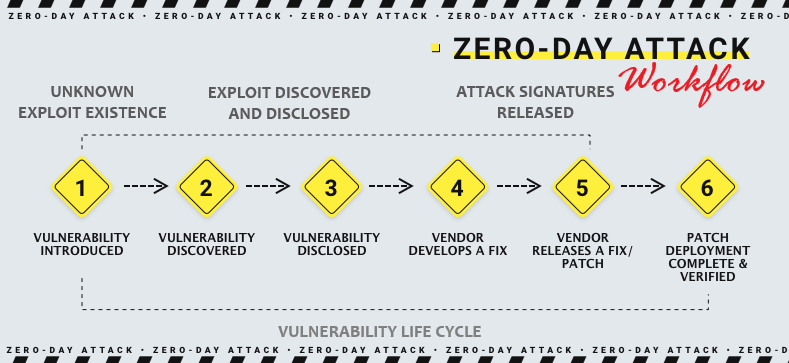
\includegraphics[width=\linewidth]{image.png}
    \caption{Enter Caption}
    \label{fig:placeholder}
\end{figure}

